\chapter{EXPERIMENTAL SETUP}
\label{chap-three}

\section*{Experimental Setup}

This chapter contains details regarding the set up of the experiment to measure absorption coefficients of various materials. The tests were performed in a Br�el \& Kj�r Impedance/Transmission Loss Measurement Tubes Type 4206A and the PULSE data acquisition software. Detailed instructions on use of the equipment can be found in Appendix \ref{append-B}.

\section{List of Materials}

\subsection{Cellulose Acetate Materials}
Many of the materials tested were provided by Eastman Chemical Company. They are as noted in the following list and as shown in Table \ref{tab:ECCsamples}. Table \ref{tab:crossSection} shows the fiber cross section.

% Small List of other materials from Eastman Chemical Company
\begin{enumerate}
    \item Several hundred white filter rods made with 2.5 DPF, Y Cross Section, 35000 total denier tow (2.5Y35000, Lot 2.5-258, tow manufactured 3/28/2014)
    \item A hand full of filter rods made with black tow
    \item A 6" by 12" sheet of cellulose acetate film made from CA-394-605 polymer
    \item Knitted Samples from Table \ref{tab:ECCsamples} below
\end{enumerate}

\begin{table}[htb]
        \caption{Fiber Cross Section Type}
        \label{tab:crossSection}
        \begin{center}
        \begin{tabular}{lcccccl}
        \toprule
        Fiber Cross Section Type & Image \\
        \midrule
        Circle & 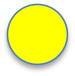
\includegraphics[width=0.07\textwidth]{Chapter-3/figs/circle} \\
        X & 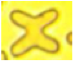
\includegraphics[width=0.07\textwidth]{Chapter-3/figs/x} \\
        Y & 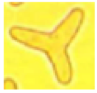
\includegraphics[width=0.07\textwidth]{Chapter-3/figs/y} \\
        8 Leg & 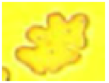
\includegraphics[width=0.07\textwidth]{Chapter-3/figs/eightleg} \\
        \bottomrule
        \end{tabular}
        \end{center}
\end{table}

% Landscape page of Samples from Eastman Chemical Company
\newgeometry{margin=1in,lmargin=1.25in,footskip=\chapterfootskip, includehead, includefoot}
    %\thispagestyle{lscape}
    %\pagestyle{lscape}
    \thispagestyle{lscapedplain}
    \begin{landscape}
    \begin{table}
        \caption{Eastman Chemical Company Samples}
        \label{tab:ECCsamples}
        \begin{center}
        \begin{tabular}{lcccccl}
        \toprule
        Sample Number & Composition & Total Denier & DPF & No. of Filaments & Fiber Cross Section\\
        \midrule
        EX1054-15-1-SOCK & Nylon & 200 & 5.9 & 34 & Round \\
        EX1054-15-2-SOCK & PET & 220 & 6.3 & 35 & Round \\
        EX1054-15-3-SOCK & Glass & 600 & 5 & 120 & Round \\
        \midrule
        EX1054-9-5-SOCK & Cellulose Acetate (TiO2) & 1576 & 2 & 788 & Y \\
        EX1054-9-1-SOCK & CA (TiO2) & 152 & 4 & 38 & Y \\
        EX1054-9-6-SOCK & CA (TiO2) & 1788 & 6 & 298 & Y \\
        EX1153-8-2-SOCK & CA (TiO2) & 1800 & 3 & 600 & Y \\
        EX1054-9-8-SOCK & CA (TiO2) & 170 & 2 & 85 & 8 Leg \\
        EX1054-9-9-SOCK & CA (TiO2) & 152 & 4 & 38 & 8 Leg \\
        EX1054-9-3-SOCK & CA (TiO2) & 150 & 6 & 25 & 8 Leg \\
        EX1054-18-1-SOCK & CA (no colorants) & 150 & 4 & 38 & 8 Leg \\
        EX1054-18-2-SOCK & CA (black colorant) & 150 & 4 & 38 & 8 Leg \\
        EX1054-18-3-SOCK & CA (TiO2) & 1800 & 4 & 450 & X \\
        EX1054-18-4-SOCK & CA (TiO2) & 1800 & 6 & 300 & X \\
        \bottomrule
        \end{tabular}
        \end{center}
    \end{table}
    \end{landscape}
    %\newgeometry{margin=1in,lmargin=1.25in,footskip=\chapterfootskip, includehead, includefoot,landscape=false}
    \restoregeometry
    \pagestyle{fancy}
    \thispagestyle{fancy}
\newgeometry{margin=1in,lmargin=1.25in,footskip=\chapterfootskip, includehead, includefoot}

% Figure of Socks from Eastman Chemical Company
\begin{figure}[hbtp]
    \centering
    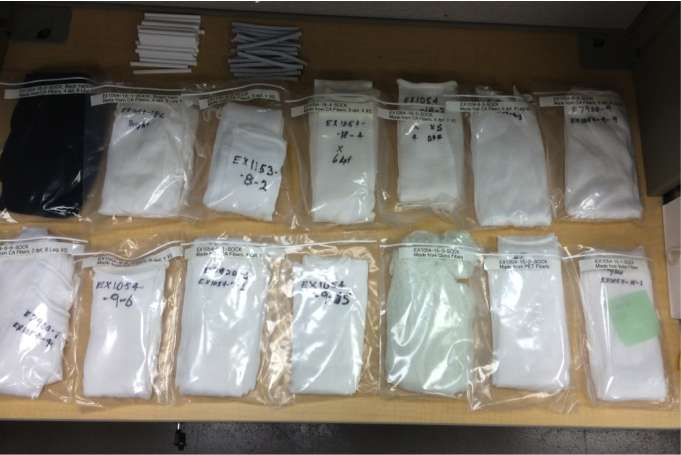
\includegraphics[width=1\textwidth]{Chapter-3/figs/ECCsocks}
    \caption{Sock Samples and Filter Rods provided by Eastman Chemical Company}
    \label{fig:ECCsocks}
\end{figure}

Above in Figure \ref{fig:ECCsocks} are all the Sock, Filter Rod, and Raw Tow materials provided by Eastman Chemical Company. Each part number provided different physical quality of Acetate Tow as shown in Table \ref{tab:ECCsamples}. 

\subsection{Commercial Materials}
In addition to Cellulose Acetate materials, commercial materials of various types were analyzed to compare to the Cellulose Acetate materials of similar type. The list of commercial materials tested is shown below.

\begin{enumerate}
	\item Sock Materials
		\begin{enumerate}
			\item Fiberglass Sock
			\item PET Sock
			\item Nylon Sock
		\end{enumerate}
	\item Raw Material Type
		\begin{enumerate}
			\item Raw Cotton Balls
			\item Auralex Compressed Cotton
		\end{enumerate}
	\item Acoustic Foam Type
		\begin{enumerate}
			\item Br�el \& Kj�r Foam
			\item Auralex Acoustics Foam
		\end{enumerate}
	\item Acoustic Panneling Type
		\begin{enumerate}
			\item Owens Corning Fiberglass Panel
			\item	Auralex Compressed Polyester Panel
		\end{enumerate}
\end{enumerate}

\section{Material Preparation for Testing}

\subsection{Sock Material Testing and O-ring}
The Sock type materials presented a challenge when testing impedance tube system. Due to the nature of the manufacture of the Sock, the materials would not lay flat on the testing surface without support. To appropriately support the woven sock type materials in the Impedance tube system, the materials were stapled to a 70-dura rubber O-ring. This method was found to be the best to prevent air gaps between the sample and the backing plate. The structural O-ring provided a means for the fabric materials to not 'curl up' in the testing area in order to get a proper measurement. This was done for each size of the Impedance tube system at 100mm and 29mm. The figure below shows a woven sock attached to the 100mm O-ring. 
\begin{figure}[hbtp]
    \centering
    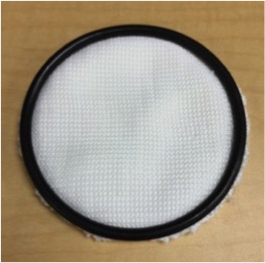
\includegraphics[width=0.4\textwidth]{Chapter-3/figs/sockOring}
    \caption{Sock Sample attached to 100mm O-ring}
    \label{fig:sockOring}
\end{figure}
In order to build a relationship regarding the thickness of the material, each Sock was tested in 4 and 8 layer configurations. In certain cases where the specific materials weight was analyzed, a sample with a different number of layers was made and tested.\\
\indent The commercial Sock materials and Cellulose Acetate Sock materials were both tested using this method.

\subsection{Cellulose Acetate Filter Rod Materials}
Tests on Cellulose Acetate as manufactured into filter rods were performed. These were performed in 2 thickness: $1.33"$ and $2.66"$ in order to build a relationship regarding the thickness of the material. A second set of rods was made with the paper removed from the samples. Due to the shape of the filter rods, it was impractical to perfectly fit them into the testing section of the Impedance Tube. For this reason the 70-dura rubber O-ring was used to create a packed array of filter rods as seen in the figure below.
\begin{figure}[hbtp]
    \centering
    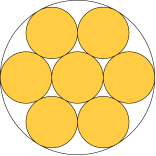
\includegraphics[width=0.2\textwidth]{Chapter-3/figs/CircleInCircle}
    \caption{Filter Rod Packing}
    \label{fig:CircleInCircle}
\end{figure}

\subsection{Raw Material Testing}
Tests on the raw cotton, and raw Cellulose Acetate provided were performed. In order to make each test consistent, the materials were weighted using clumped balls of $1.5$ grams. Five balls of equal weight were oriented into the machine, tested, and then averaged. This was done for the raw cotton balls and the raw Cellulose Acetate materials

\section{Impedance Tube Testing}

\subsection{Sample Preparation}
Each Sock sample was attached to an O-ring before it was loaded into the impedance tube testing section. Multiple layers of each Sock was created. 4 layers and 8 layers can be seen in the data shown in Chapter \ref{chap-four}.

\subsection{Setup}
Materials were configured for the 100mm and 29mm tubes. However, due to material limitations, all samples were tested in the 100mm tube. It is important to note that the smaller tube covers a broader range of frequencies, 500Hz to 6.3Hz, and hence dictates much better information about the overall performance of the material.

\subsection{Software}
Once the hardware and materials were properly configured, testing procedure continued on the attached laptop running PULSE software provided by Br�el \& Kj�r. Full details regarding the software can be found in Appendix \ref{append-B}.

\subsubsection{PULSE Software}
The PULSE software was used to collect data from the impedance tube system. The software was initialized, calibrated, and run in each test on every material. Each material was tested $5$ times and averaged to reduce hysteresis effects. The presented data in Chapter \ref{chap-four} is the averaged data. The data collected by the software was then exported into a spreadsheet file to be post-processed in MATLAB.

\subsubsection{MATLAB Software}
All data exported from PULSE was imported into MATLAB for analysis and graphical processing. The MATLAB scripts used for processing can be found in Appendix \ref{append-C}. Resultant graphs can be found in Chapter \ref{chap-four}.
